\RequirePackage{fix-cm}
\documentclass[smallextended]{svjour3}
\smartqed
\usepackage{amsmath,amssymb,graphicx,booktabs,array,longtable}
\usepackage[numbers,sort&compress]{natbib}
\usepackage{url}
\usepackage{float}
\floatstyle{ruled}
\newfloat{algorithm}{tbp}{loa}
\floatname{algorithm}{Algorithm}
\usepackage[hidelinks]{hyperref}
\journalname{Autonomous Agents and Multi-Agent Systems}
\newcommand{\E}{\mathbb{E}}
\newcommand{\U}{U}
\newcommand{\ind}{\mathbf{1}}
\newcommand{\authorinput}[1]{\textbf{AUTHOR INPUT NEEDED: #1}}
\setlength{\emergencystretch}{3em}
\raggedbottom
\clubpenalty=10000
\widowpenalty=10000
\hypersetup{pdftitle={Auditing the Value of Delayed Advice in Autonomous Agents}}
\begin{document}
\title{Auditing the Value of Delayed Advice in Autonomous Agents}
\titlerunning{Auditing the Value of Delayed Advice}
\author{Author information pending}
\authorrunning{Author information pending}
\institute{Author names, affiliations and correspondence must be supplied before submission.}
\date{}
\maketitle
\begin{abstract}
Autonomous agents often continue acting while an expert reply is delayed. An improved policy can then be mistaken for evidence that the returned information was useful. We present a simulation evaluation framework that separates fitted-pipeline performance, runtime message dependence and the outcome value of a specified message channel. The protocol freezes policies, records decisions before outcomes, executes paired native trajectories and audits replay. In visual manipulation, a packet-input variant improved PickPlace reward by 0.735 over its local-input counterpart, yet its selected predictor was identically zero and rejected every intervention. The gain therefore did not require the newly returned message. A new channel experiment freezes the original visual system on 60 nonzero-delay environments: refreshing changes decisions and actions, but its reward difference from stale delivery remains unresolved. Defined stale, refreshed and absent channels on 180 further state-task environments provide complementary outcome evidence. An independent timestamp-decoder control improves a fixed fresh chunk relative to stale-offset decoding, without establishing a selector benefit. Finite-pool diagnostics distinguish available action opportunity from harmful selection; three complete visual training systems assess randomness conditional on shared data and pretraining. These findings support an executable evaluation discipline: performance, dependence and channel value require different evidence. They do not establish that delayed advice improves robot performance, that expert information is generally ineffective, or that the results transfer to private observations, real asynchronous services or hardware safety.
\keywords{Autonomous agents \and Action advising \and Delayed feedback \and Counterfactual evaluation \and Reproducibility}
\end{abstract}
\section{Introduction}\label{sec:intro}
An autonomous agent can continue acting while advice is computed or communicated. When a reply arrives, the agent faces two questions: whether to change its behavior, and whether any resulting improvement can be credited to the information in that reply. The second question is easily obscured by the first. A policy trained with advice features may outperform a policy trained without them because fitting or model selection changes, even when the final deployed decisions do not depend on those features.

Action advising has long distinguished what to teach, when to teach and how a learner uses advice. Teacher quality and student benefit need not have a simple relationship~\cite{fachantidis}; demonstrations, corrections and guidance enter a learner through different mechanisms~\cite{najar}. Confidence-based autonomy regulates requests for demonstrations~\cite{chernova}, while advice reuse and imitation transfer teacher knowledge into the student~\cite{zhu,ilhan}. These results make offline knowledge and online communication distinct parts of an advice system. They also motivate a precise evaluation question: when two advice-labelled pipelines obtain different rewards, does the deployed behavior actually depend on the returned message?

Delayed control sharpens the attribution problem. Action Chunking with Transformers (ACT) predicts sequences from demonstrations~\cite{act}, and real-time chunking addresses asynchronous execution for flow-based policies~\cite{rtc}. Yet a capable complete-episode source need not be a useful occasional advisor to an already competent local controller. At arrival, a selector may change a local action, execute source actions, or reject. A feature-availability ablation can simultaneously change representation, fitted coefficients and validation selection. Its reward difference is therefore a whole-pipeline result unless additional controls establish the role of the runtime message.

We study this issue through a simulation evaluation framework for delayed advice in autonomous decision making. The framework makes the target contrast explicit, retains executable local and null-advice references, records decisions before counterfactual outcomes, and checks native branch replay. Its central empirical case is a positive packet-input-labelled reward contrast whose selected policy is identically zero and always rejects intervention. This is a concrete counterexample to a particular attribution, rather than evidence that advice is generally ineffective. A simple dependency certificate explains why its behavior can be reproduced without a returned packet.

The paper contributes three connected elements. First, it distinguishes fitted-pipeline performance, fixed-policy message dependence and value under a specified channel intervention, with an elementary counterexample and an observed executable null policy. Second, it turns those distinctions into an operational audit: a workflow, an algorithm, pre-outcome decisions, native branch replay and explicit message-generation/fallback rules. Third, it supplies the visual attribution counterexample on two manipulation tasks and direct fixed-policy channel outcomes on the original frozen visual PickPlace system and three state-observation contact tasks, with finite-pool diagnostics that distinguish limited opportunity from harmful selection. Further experiments examine critic data, training variation, delay, sensor noise, request schedules and model-selection tolerance. The contribution is an evaluation framework and its empirical failure mechanisms; standard regression, null models and matched branching are established components, not claimed algorithmic inventions.

The agent-level relevance is methodological. Teacher--student and decision-support architectures are often evaluated through end-to-end reward. Establishing an improvement remains necessary, but identifying its origin requires checking what the deployed system consumes and comparing outcomes under a defined intervention. Our implementation uses a single learner and a fixed computational advisor; it does not demonstrate strategic multi-agent interaction. The abstract distinction applies beyond robotics, while its empirical support here remains limited to simulated manipulation.

\section{Related work}\label{sec:related}
\subsection{Action advising, teaching and retained expertise}
Budgeted action advising allocates a teacher's finite opportunities to help a learner~\cite{torrey}. Fachantidis et al.~\cite{fachantidis} study teaching characteristics and learned advising, demonstrating why a teacher's own task competence and its teaching effectiveness are different quantities. Confidence-based autonomy regulates demonstration requests and corrections~\cite{chernova}. Policy shaping integrates noisy human feedback as policy information~\cite{griffith}, whereas policy-dependent feedback changes meaning with the learner's behavior~\cite{macglashan}. Corrective continuous-action teaching additionally addresses how a delayed correction is assigned to earlier behavior~\cite{celemin}. These are substantive mechanisms for obtaining and integrating advice; our frozen-deployment audit does not replace their learning objectives.

Advice reuse and behavioral imitation can transfer teacher knowledge into a student that later acts without a new message~\cite{zhu,ilhan}. Single-agent and multi-agent transfer surveys place such retained expertise in a broader knowledge-transfer setting~\cite{taylor,silva}; Najar and Chetouani~\cite{najar} distinguish the forms and integration of human advice. Accordingly, our null-policy certificate concerns dependence on the \emph{newly returned} message, not the absence of expert influence in demonstrations, pretrained representations or fitted parameters. A query-free deployed controller may still embody substantial offline expertise.

Recent preprints refine adjacent questions. Pugnana et al., \emph{To Ask or Not to Ask: Learning to Require Human Feedback} (2025, \url{https://arxiv.org/abs/2510.08314}), study feedback acquisition for prediction. Alur et al. (2024, \url{https://arxiv.org/abs/2410.08783v2}) formalize expert complementarity using algorithmic indistinguishability, a stronger information setting than our deterministic public-source messages. Shihab et al. (2026, \url{https://arxiv.org/abs/2609.29548v2}) distinguish returned advice, executed actions and matched-budget acquisition value. We do not claim to originate these distinctions. Their reported language-model settings and guarantees are not reproduced here.

\subsection{Latency, asynchronous control and action chunks}
Real-world reinforcement learning faces delays alongside partial observability and other deployment constraints~\cite{dulac}. Real-time reinforcement learning explicitly lets the environment evolve during agent computation~\cite{ramstedt}; random-delay reinforcement learning develops delay-aware trajectory treatment~\cite{randomdelay}. ACT and Diffusion Policy learn temporally extended visuomotor actions~\cite{act,diffusion}, while real-time chunking preserves execution consistency during asynchronous chunk generation~\cite{rtc}. These methods seek effective control under their respective timing models. Synthetic native-step delays in this study isolate an attribution question; they do not reproduce live network or inference-service latency.

The PACT-VLA preprint (Zhu et al., 2026, \url{https://arxiv.org/abs/2610.28019v1}) uses pre-commit observations to select chunks. Appendix D.2 already selects from fixed candidate pools before branch rollout with a common continuation controller. Matched branching is therefore a precedent, not a novelty claim of this paper. Our framework combines that experimental logic with an executable null certificate and separately defined policy, dependence and channel contrasts. Sequential imitation also changes the visited-state distribution~\cite{ross}; this motivates distinguishing a common arrival snapshot from later states that diverge after intervention.

\subsection{Counterfactual evaluation and message dependence}
Off-policy evaluation estimates a policy's value from previously logged behavior. Doubly robust methods combine outcome and propensity information~\cite{dudik,jiang}, and sequential estimators address data efficiency~\cite{thomas}. Counterfactual risk minimization instead uses logged bandit feedback to learn policies with controlled risk~\cite{swaminathan}. Our framework executes the declared counterfactual trajectories in a restorable simulator. It is not a new logged-data estimator and cannot remove support requirements when native branching is unavailable.

Model reliance studies distinguish the behavior of one fitted model from that of other similarly accurate models~\cite{fisher}. Unrestricted feature permutation can force extrapolation~\cite{hooker}, while conditional importance treats dependencies between predictors explicitly~\cite{strobl}. These results are especially relevant when an expert message is a deterministic function of public observations. Changing a packet may test a model's response to that input but does not, by itself, identify information value on the training distribution. Our native channel experiment therefore defines a real message provider and a missing-message wrapper in advance; it reports the resulting controlled channel contrast with its joint-input distribution limitation.

\subsection{Selection, reproducibility and the remaining gap}
Model selection can overfit its evaluation criterion~\cite{cawley,varma}; training seeds, implementation choices and small-run uncertainty can alter reinforcement-learning comparisons~\cite{henderson,agarwal}. Reproducible research requires accessible experimental and implementation evidence~\cite{pineau}. We preserve whole-episode splits, validation selection rules, null candidates, pre-outcome decisions and replay checks. These are established safeguards. The framework's additional target is semantic: a well-estimated reward gap between selected pipelines may still fail to identify the role of a message at deployment.

Table~\ref{tab:related} makes the narrower comparison explicit. It is a protocol comparison, not a priority proof or an assessment of the cited methods' overall quality. The contribution is the integrated, executable audit and its measured attribution counterexample, now connected to fixed-policy native channel outcomes and finite-pool failure diagnostics.
\begin{table}[tb]\centering\small
\caption{Relation to representative work. D: delayed messages/actions; M: fixed-policy message replacement; N: executable no-advice reference; B: paired native branches from a common snapshot; V: direct outcome contrast between specified message channels of the same policy. ``NR'' means not established in the reviewed material, not proof of absence; ``--'' is outside that work's scope. N includes ordinary no-advice controls and does not imply an algebraic null certificate.}\label{tab:related}
\setlength{\tabcolsep}{4pt}
\begin{tabular}{p{6.1cm}ccccc}\toprule Representative setting & D & M & N & B & V\\\midrule
Budgeted advising~\cite{torrey,fachantidis} & NR & NR & Yes & NR & NR\\
Corrective continuous-action teaching~\cite{celemin} & Yes & NR & NR & NR & NR\\
Real-time/random-delay RL~\cite{ramstedt,randomdelay} & Yes & NR & -- & NR & NR\\
Logged-data policy evaluation~\cite{dudik,jiang,thomas} & -- & -- & -- & -- & --\\
PACT-VLA, Appendix D.2 (preprint) & Yes & NR & Yes & Yes & NR\\
Present native channel study & Yes & Yes & Yes & Yes & Yes\\\bottomrule
\end{tabular}
\end{table}

\section{Problem formulation}\label{sec:formulation}
\subsection{A delayed-advice decision process}
Consider an autonomous agent with observation history $H_t$, native state $S_t$, action $u_t$ and exogenous randomness $\omega$. An advisor generates $M_q$ using the permitted request observation at native step $q$. Local control continues until arrival $a=q+d$. A frozen arrival policy then chooses an option from a declared finite family; each option has a fixed execution rule and returns to the specified continuation controller after its intervention window. A common continuation \emph{controller} may take different future actions on the different states reached by the branches.

We use complete-episode utility
\begin{equation}
 U_\omega(\pi)=\frac{1}{T}\sum_{t=0}^{T-1}r_t,\qquad T=500,\quad 0\leq r_t\leq10.
\end{equation}
Thus, the archived \texttt{native\_return} is a mean, not an unnormalized return. Native any-success and terminal-success are separate secondary outcomes. The simulator reward scale does not make an equal difference operationally interchangeable across tasks. Table~\ref{tab:notation} fixes the notation used throughout the paper.
\begin{table}[tb]\centering\small
\caption{Notation and evaluation roles. Channel labels are distinct from the $C/F$ action-set labels.}\label{tab:notation}
\begin{tabular}{lp{.72\textwidth}}\toprule
Symbol & Meaning\\\midrule
$q,d,a$ & Request step, delay in native steps, and arrival $a=q+d$\\
$M_q$ & Message generated from the request information\\
$g$ & Message generation step, supplied to the separate timestamp-aware decoder\\
$u_t,U$ & Native action and mean reward over all 500 steps\\
$R$ & Reject intervention and continue the unchanged local controller\\
$L/P$ & Local inputs / local inputs plus the returned packet\\
$C/F$ & Local option family / full family including source actions\\
$\pi,\bar\pi$ & Frozen present-message policy / fixed wrapper with an explicit missing-message rule\\
$c_s,c_f,c_\emptyset$ & Stale-request, arrival-refresh and erased-delivery channels\\
$\epsilon_{\rm tie}$ & Tolerance used during development-model selection\\
$\tau_{\rm accept}$ & Deployment threshold on predicted intervention gain\\
$H_{\mathcal O},G_\pi$ & Finite-pool oracle headroom and selection regret\\\bottomrule
\end{tabular}\end{table}

\subsection{Pipeline performance, dependence and channel value}
The first question concerns the performance of entire training pipelines. Let $\mathcal A_L(D)$ and $\mathcal A_P(D)$ include normalization, fitting, validation and numerical tie-breaking with and without packet features. Conditional on the fitted policies,
\begin{equation}\label{eq:pipeline}
 \Delta_{\rm pipe}=\E_\omega[U_\omega(\mathcal A_P(D))-U_\omega(\mathcal A_L(D))].
\end{equation}
Changing feature availability may change coefficients or even the selected model class. This legitimate pipeline-performance estimand does not hold the deployed decision rule fixed.

The second question is behavioral dependence: with the frozen policy and nonmessage inputs held fixed, can changing a message change an option choice or executed action? Both routes matter. A packet-input gate may select only local actions, while a local-input gate can select an expert option whose actuator commands directly consume the packet. Choice invariance alone is therefore insufficient to certify action invariance.

The third question requires an explicitly defined channel intervention. For a frozen policy and channels $\mathcal P,\mathcal Q$, define
\begin{equation}\label{eq:channel}
 \Delta_{\rm ch}(\pi;\mathcal P,\mathcal Q)
 =\E_{\omega,M\sim\mathcal P,\widetilde M\sim\mathcal Q}
 [U_\omega(\pi;M)-U_\omega(\pi;\widetilde M)].
\end{equation}
The conditioning and coupling of the messages, request clock, continuation and cost convention are part of the estimand. Repeated requests can generate different future states and messages under different channels, requiring complete closed-loop evaluation rather than repeated forced alignment of histories.

Our channel experiments estimate specified refresh and availability contrasts. Channel $c_s$ applies the original expert to the noisy request observation; $c_f$ applies the \emph{same} expert to the noisy arrival observation, with no extra simulated refresh latency. Writing the public source as $e$ and its permitted noisy observation as $\widetilde O$, the channels return $M_q^S=e(\widetilde O_q)$ and $M_q^F=e(\widetilde O_a)$; the request identity $q$ and nonmessage clock features stay fixed. Here $d$ remains elapsed request delay, rather than the generation age of the intervened refreshed message. Both retain the same message encoding (one four-dimensional action for state sources; a 100-action packet for visual ACT) and candidate functions. Channel $c_\emptyset$ returns an absent-message symbol, not a zero vector. Because the original trained gate has no missing-input interface, we declare a fixed evaluation wrapper before testing:
\begin{equation}\label{eq:wrapper}
 \bar\pi(x,M)=\begin{cases}R,&M=\varnothing,\\\pi(x,M),&M\neq\varnothing.\end{cases}
\end{equation}
The original present-message coefficients and thresholds remain unchanged. This totalization is an evaluation convention, not a claim of learned robustness to missing messages. Comparing $\bar\pi$ under $c_s,c_f,c_\emptyset$ isolates these defined channel effects under the simulator assumptions. Queries and prefix clocks remain forced; erasure does not measure saved acquisition cost.

These contrasts do not identify intrinsic information value. The implemented packets are deterministic functions of request or arrival inputs already in the permitted local information set, conditional on fixed expert weights. They may supply a useful computation to a restricted learner without adding a private measurement. Moreover, the refreshed packet changes its joint relationship with the nonmessage inputs relative to stale-only training. Actual source generation makes the intervention interpretable; it does not establish that the resulting joint inputs are in distribution. We therefore report a controlled refresh-channel effect, not a distribution-free claim about expert information. Arbitrary packet scrambling would answer yet another question~\cite{hooker,strobl}.

\section{The delayed-advice audit framework}\label{sec:framework}
\subsection{An executable evaluation procedure}
The framework turns the three questions into separate audit routes (Fig.~\ref{fig:workflow}; Algorithm~\ref{alg:audit}). Models, option functions and statistical comparisons are frozen before test environments are opened. Source competence is assessed separately from its marginal contribution at arrival. Local references include continued local control and development-selected fixed options; a hindsight-best option is never presented as executable assistance.
\begin{figure}[tb]\centering
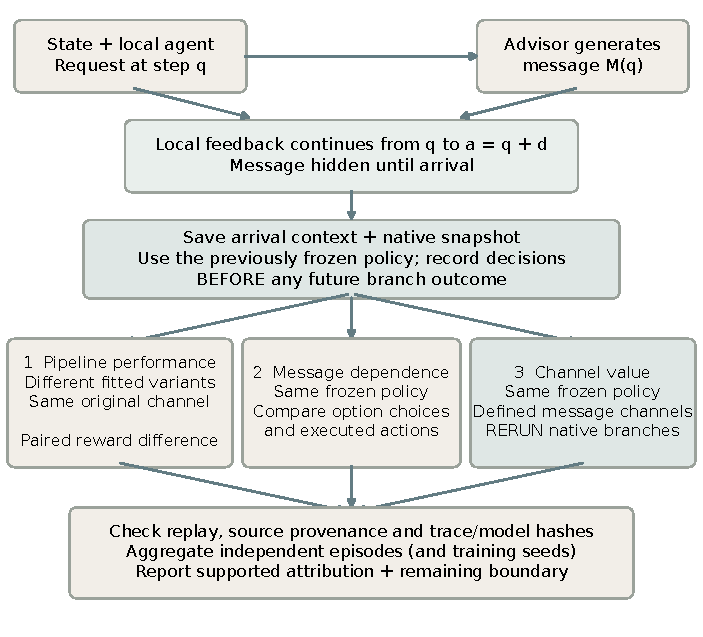
\includegraphics[width=\textwidth]{figures/advice_audit_workflow.pdf}
\caption{The delayed-advice audit workflow. Local control advances while a message is unavailable. At arrival, choices are logged before future outcomes. Pipeline comparisons use different fitted variants; dependence checks inspect choices and commands of a fixed policy; channel-value tests rerun actual native branches under defined message mechanisms. Replay and provenance checks precede attribution.}\label{fig:workflow}
\end{figure}
\begin{algorithm}[tb]
\caption{Delayed-Advice Audit Procedure}\label{alg:audit}
\small
\textbf{Inputs:} local controller, advisor, trained arrival policies, message channels, delay/query protocol, option functions, continuation, held-out environments and exogenous seeds.\par
\begin{enumerate}
\item Specify $U$, costs, $T$, splits, primary contrasts, uncertainty method, and the conditioning of each channel. Define missing-message behavior explicitly.
\item Fit/select only on development episodes, or reuse verified trained policies. Freeze weights, normalization, thresholds, option functions and source hashes.
\item For each held-out episode, run local control to $q$, generate the permitted request message, and continue locally to $a=q+d$ without exposing it early.
\item Save the arrival snapshot and permitted nonmessage context. Generate each control message only from its declared observation/time information.
\item For every frozen policy and channel, log inputs, message provenance, scores and the selected option \emph{before} any branch outcome is observed.
\item Restore the common snapshot and execute each required option/message branch through its repair window and common continuation to $T$. Reuse a trace only for an exactly identical executable plan. Evaluate all options only when an offline headroom diagnostic is declared.
\item Check complete replay, hashes, source-message consistency, trajectory lengths and agreement between saved choices, actions and rewards. Report failures instead of silently excluding episodes.
\item Estimate pipeline contrasts separately from fixed-policy channel contrasts. Record both decision and command changes. Resample complete environments and training seeds as required, not correlated option branches.
\item Report the supported attribution, channel/support/cost boundary and finite-pool diagnostics. If no outcome-valid channel intervention was executed, leave $\Delta_{\rm ch}$ unestimated.
\end{enumerate}
\textbf{Outputs:} auditable performance contrasts, dependence diagnostics, defined channel-value estimates where available, and a claim-boundary record.
\end{algorithm}

For a single arrival, compared branches share the request trajectory, fixed arrival context and future exogenous noise. Their intervened messages and option selections may differ. Each branch executes its actual native action rule and then returns to the same continuation controller. Complete episodes define train/validation/test groups and resampling units. Snapshots, branch rewards and native prefix success are excluded from policy features.

Counterfactual consistency requires restoring more than generalized coordinates. Our snapshot includes full MuJoCo integration and derived data, Python-side task state, observation history, reward bookkeeping, relevant model arrays, random state and aliases into native arrays. Copying an aliased view into a detached array can change reward semantics. Under the declared renderer, complete-tail checks compare images, predictions, actions, rewards and success labels. These checks establish local consistency, not universal simulator or hardware determinism.

\subsection{An executable null-advice certificate}\label{sec:null}
A zero gain predictor makes one dependency case inspectable. Let every nonreject option and reject have predicted gain zero, and intervene only when the selected gain exceeds a positive threshold. The deployed gate then always returns $R$.
\begin{proposition}\label{prop:null}
Suppose a frozen arrival policy always rejects and its continuing local controller does not consume returned messages. If queries do not affect physical transitions, observations or local-controller resources, replacing or removing the messages preserves every action and reward under the same initial state and exogenous randomness.
\end{proposition}
\begin{proof}
Before arrival, the histories and local actions agree. At arrival both implementations select $R$. Their next local actions agree, and coupled transition/observation functions give the same next histories. Induction through the remaining steps and any further scheduled arrivals proves equality.\qed
\end{proof}
An instrumented evaluator may still generate, serialize or normalize a packet before returning the zero decision. The certificate concerns functional action/reward dependence and an equivalent packet-free implementation, not an observed saving in message-processing time. This is a simple dependency argument, not a new control theorem. Real queries can consume shared compute or human attention, violating its assumptions. Our forced-query simulator does not measure such savings.

A finite example explains the attribution problem. In one known state, two executable local actions have rewards 0 and 1; the continuation chooses the latter. A fitted local-input variant mistakenly intervenes with the former, whereas a packet-input pipeline selects the zero predictor and rejects. Its pipeline advantage is 1 for any returned message, including an irrelevant constant, but the winning policy has no runtime message dependence. A positive $\Delta_{\rm pipe}$ is therefore compatible with zero channel effect. The implemented visual study tests whether this possibility occurs in an actual learning pipeline.

\subsection{Diagnosing opportunity and selection separately}
The audit crosses local/packet inputs ($L/P$) with local/full option families ($C/F$). The resulting separately fitted contrasts $P,C-L,C$, $P,F-P,C$ and $P,F-R$ describe pipelines; they are not a causal decomposition or the benefit of an optimally used action set.

When all predeclared options are rerun, a finite-pool offline diagnostic separates opportunity from selection. At a fixed snapshot and channel, let
\begin{align}
 H_{\mathcal O}&=\max_{o\in\mathcal O}U(o)-U(R),\\
 G_\pi&=\max_{o\in\mathcal O}U(o)-U(o_\pi).
\end{align}
Because $R\in\mathcal O$, $H_{\mathcal O}\geq0$ and the exact identity
\begin{equation}\label{eq:regret}
 U(o_\pi)-U(R)=H_{\mathcal O}-G_\pi
\end{equation}
holds. Small $H_{\mathcal O}$ limits improvement within the tested family; a large $G_\pi$ identifies missed opportunity or harmful selection. Comparing $\max_{\mathcal O_F}U$ with $\max_{\mathcal O_C}U$ further measures source-exclusive finite-pool headroom. None is a deployable policy, an upper bound over all possible controls, or an online regret guarantee.

This protocol also sets a minimum reporting standard beyond robotics: identify which inputs and models changed; specify where expert knowledge already exists offline; define the timing and provenance of each message; make absence and continuation executable; and measure actual outcomes for the claimed channel comparison. Without a rollback-capable simulator or equivalent experimental design, branch values cannot be recovered from decision sensitivity alone. Logged-data policy evaluation offers a separate route with its own overlap and estimation assumptions~\cite{dudik,jiang,thomas,swaminathan}.

\section{Experimental design}\label{sec:design}
Table~\ref{tab:studies} separates observation regimes and training variation. All studies use Meta-World~\cite{metaworld} 3.1.1/MuJoCo 3.3.0, a native 500-step horizon and mean native reward $U\in[0,10]$. Any-success records at least one native success event; terminal-success records the final step. Option branches and repeated policies are not independent environments. Online Resource 1 retains full training, condition, replay and provenance details.
\begin{table}[tb]\centering\small
\caption{Study roles and distinct observation/training regimes. Test counts are independent initial environments, not option branches or model--environment records. Actors and critic seeds vary different components. The full visual replication reuses 40 original development initial environments across three systems.}\label{tab:studies}
\setlength{\tabcolsep}{3pt}
\begin{tabular}{p{3.1cm}p{3.5cm}p{2.9cm}r}\toprule Study & Tasks / observations & Training variation & Test $n$\\\midrule
Original visual & Push, PickPlace / RGB+robot & Actor seed 0 & 500\\
Critic-data curve & Same visual tasks & Critic data 7/14/28 & 200\\
Full visual replication & Same visual tasks & Full systems 0/1/2 & 100\\
State stress suite & Drawer, Door, Button / state & Five critic seeds & 360\\
State channels & Same state tasks & Same frozen critics & 180\\
Visual channels & PickPlace / RGB+robot & Frozen original seed 0 & 60\\
Decoder control & PickPlace / RGB+robot & Same models; changed executor & 60\\\bottomrule
\end{tabular}
\end{table}


\subsection{Visual policies and development}
Push and PickPlace actors receive a vertically flipped $512\times512$ corner4 RGB image and four robot coordinates, without online object/goal poses. The ACT source~\cite{act} uses a pinned public pretrained initialization and produces 100 four-dimensional actions; it is not language-conditioned. Four local action/pose heads share a frozen ResNet-18 encoder. Each task supplies the same 200 demonstrations, split by whole episode into 180 training and 20 validation. Heads train for 20 epochs; ACT trains for 15,000 updates with validation-only checkpoint selection. Deployment capacities remain fixed. Pose heads receive additional offline supervision, so this is not an equal-information architecture comparison.

The original source reached any-success in 79/100 Push and 83/100 PickPlace qualification episodes, versus 91/100 and 90/100 for the selected local controllers. This establishes competence, not occasional-advice value. The seven local options comprise reject, three alternative feedback heads, an ensemble and request/arrival action holds; the full family adds five ACT prefix/suffix/blend options. Online Resource 1 specifies their execution rules.

The original arrival pool has 20 independent development episodes/task (14 training, six validation). Standard RBF kernel ridge critics predict option gains from request/arrival feature maps, robot coordinates, all head predictions and clocks; $P$ adds the full packet. Validation selects among 12 bandwidth/ridge combinations and zero. A $10^{-12}$ global-MSE tie tolerance favors zero; deployment requires predicted gain above $10^{-12}$. Actors and all four $L/P\times C/F$ critics are frozen before testing. Counterfactual rendering uses MSAA0 to remove observed same-state image variation; historical training features used MSAA4. This recorded change remains a distribution limitation.

\subsection{State policies and stress conditions}\label{sec:state-design}
Drawer, Door and Button cover sliding, hinged motion and pressing. They use ten public coordinates (hand, gripper, object and goal), a deterministic public scripted source and a nearest-neighbor behavioral-cloning local controller, rather than visual ACT. A preassigned demonstration ladder selects 40 episodes/task and $k=1,5,1$ using separate validation. Independent qualification requires both actors' any-success at least 0.8 on 20 environments; all three tasks pass and remain included.

Each task supplies 42 single-arrival development episodes (30/12 split). Six local options comprise reject, two alternative feedback policies and three action holds; four additional options hold or blend the source action. Five independently initialized 64/32 tanh critics per input/action cell train for 1,000 updates with validation checkpoint selection and an eligible zero predictor. Feature dimensions are 58/62; the tie tolerance is $10^{-12}$ and acceptance threshold $10^{-8}$. These are critic seeds around fixed actors, not independent actor-training systems.

A separate 360-environment stress suite crosses delays 0/16/64, single/periodic requests and position-noise standard deviations 0/0.005 m (120 environments/task). Noise affects nine position coordinates, with common time-indexed streams across branches. Periodic requests cannot overlap intervention windows. Packet zeroing, negation and reversal are gate-sensitivity probes only: no rerolled outcome or in-distribution interpretation is assigned to them.

\subsection{Fixed-policy channel studies}\label{sec:channelsetup}
Both channel studies freeze the trained receiver, normalization, thresholds, option functions and continuation. A common local prefix reaches the same arrival snapshot. Stale $c_s$ uses the source's request observation; fresh $c_f$ applies the same source to the arrival observation; absent $c_\emptyset$ invokes the fixed reject wrapper in Eq.~\eqref{eq:wrapper}. Messages are generated by the actual source, never arbitrary zero packets. Nonmessage inputs and request/delay clocks stay fixed. No extra refresh latency or acquisition cost is charged. Actual source generation does not ensure joint-input support under stale-only training.

The state study reuses all 60 critics on 60 fresh environments/task: delays 0/16/64 crossed with noise 0/0.005 m, ten per cell; a preassigned request occurs at 16/144/272/400. Every stale option and each distinct fresh source option is executed. The visual bridge instead fixes the \emph{original} seed-0 PickPlace system, connecting the null $P,C$ counterexample and the nonzero $P,F$ receiver. Its primary 60 fresh environments all have nonzero delay: 16/32 crossed with requests 16/32/64, ten per cell. Six separate delay-zero identity cases and two engineering cases are excluded from inference. Only distinct chosen plans and reject are executed, without a new oracle sweep.

For visual $c_f$, literal packet replacement retains the original option decoder, including suffix index $d+\text{elapsed}$. It does not reset fresh-message age or optimize a refresh controller. The contrast therefore tests this fixed receiver's content replacement, not the best possible refresh mechanism. Full 500-step rewards, actions and native success flags are retained. Channel choices are recorded before future outcomes; $R$ is independently replayed in every case. Decision changes and complete action differences above $10^{-8}$ are counted separately.

\subsection{Independent generation-time decoder control}\label{sec:decodersetup}
A separate experiment tests execution semantics on 60 new PickPlace environments, using the original seed-0 actors and critics without retraining. Delays 16/32 cross requests 16/32/64, with ten environments per cell; six zero-delay identities and two engineering cases are excluded. For a message generated at $g$, the time-matched suffix/blend decoder uses $(a-g)+\text{elapsed}$. Stale messages have $g=q$, reproducing the original index; refreshed messages have $g=a$, starting at zero. Raw-prefix and local options are unchanged. For the fixed 48-step option, time-matched fresh execution is the existing fresh raw-prefix candidate, not a new controller.

We evaluate both a predeclared fixed 48-step source suffix and the frozen $P,F$ gate. The gate receives unchanged packet/nonmessage features and selects the same option for both fresh decoders; only the downstream execution index changes. The four primary paired reward contrasts compare time-matched fresh execution against legacy fresh and legacy stale execution, separately for the fixed option and gate. Thirty thousand whole-environment bootstrap resamples within the six cells give approximate 98.75\% intervals for this independent four-contrast family. Secondary success and reject comparisons are descriptive.

This changes the executable receiver and therefore is an independent decoder-policy comparison, not a reinterpretation of the original fixed-policy channel effect. Since stale decoding is unchanged, fresh-versus-stale also measures refreshing under the newly defined timestamp-aware rule. The critic remains fitted to legacy outcomes; neither age-aware retraining nor optimal source timing is tested. Known, correct generation timestamps are assumed. No extra refresh latency or service cost is charged. Online Resource 1 retains the complete protocol, outcomes and index checks.

\subsection{Training variation and supporting studies}\label{sec:fullseedsetup}
The complete visual replication retains seed 0 and independently trains seeds 1/2, including ACT's full 15k budget, all four local heads and separately fitted 14/6 arrival critics. All share the immutable demonstration corpus, pretrained initialization, capacities and original development environment/clock arrangement. New actors generate their own development labels. This tests conditional training randomness, not cross-dataset or cross-task-distribution generalization.

Fifty fresh initial environments/task are shared by the three systems (100 independent initial environments, 300 system--environment cases). Every system also executes separate reset-source trajectories; none is excluded for weak competence. All 12 options are executed on the first ten preassigned environments/task per system for offline headroom. Figure~\ref{fig:scenes} illustrates excluded engineering cases rather than selected successful test episodes.

Supporting studies retain the original 250-environment/task visual confirmation, a new nested 7/14/28-episode critic-data curve with 100 fresh tests/task, and 100 development resplits across five tie tolerances. The earlier 3k source-budget studies are historical controls in Online Resource 1, not the full replication.

\subsection{Statistics, audit and research execution}\label{sec:statistics}
Comparisons retain whole-environment pairing. Stratified bootstrap resamples environments within preassigned cells; crossed versions additionally resample actor or critic seeds, never treating options as independent. The inference contract in Online Resource 1 gives every primary family, sample size and confidence level. These approximate percentile intervals have limited coverage with few training seeds or sparse differences; separate studies do not supply a global family guarantee. Native success, subgroup breakdowns and headroom are descriptive. The investigator-defined 0.25 reward reference has no validated operational meaning. Nonzero-delay state subsets are explicitly post-hoc, with exploratory 95\% intervals.

Frozen model/entry hashes, source consistency, raw reward means and recorded decisions are audited. Native restoration includes integration, task, observation-history and random state; local replay does not establish clean-machine portability. Source schedules, failed-run records and exact checks are retained in Online Resource 1. OpenAI Codex assisted implementation, orchestration, aggregation, literature checking and drafting beyond copy editing. Automated audits are not independent human verification; authors must verify and take responsibility for the final work.

\begin{figure}[tb]\centering
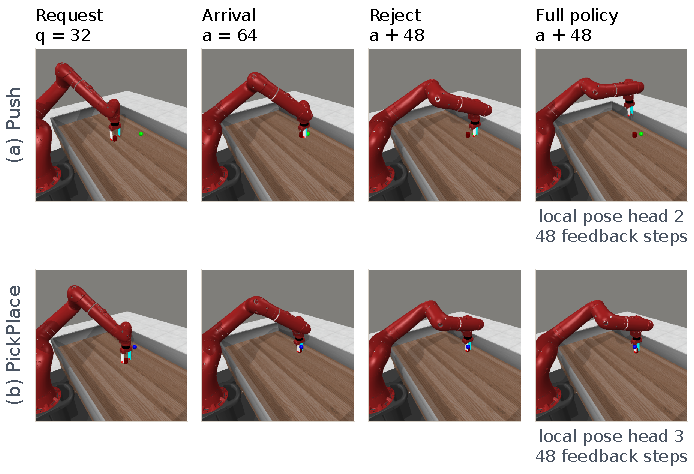
\includegraphics[width=\textwidth]{figures/simulator_scenes.pdf}
\caption{Preassigned engineering episodes, excluded from inference. Local control continues from request $q=32$ to arrival $a=64$. Final columns compare reject and $P,F$ at $a+48$. The policies select local pose heads 2 (Push) and 3 (PickPlace), not source actions. Each scene panel is rotated by $180^{\circ}$ for display; no crop or other pixel adjustment is applied. These are timing/branching examples, not efficacy evidence.}\label{fig:scenes}
\end{figure}

\section{Results}\label{sec:results}
\subsection{A positive pipeline contrast required no runtime packet}
The original visual confirmation completed all 500 scheduled environments. The packet-input/full-action policy lost reward against local continuation on both tasks (Table~\ref{tab:visual}). A separate audit reproduced all saved choices and reward means. These are results of the frozen selectors, not the quality of every possible expert intervention.
\begin{table}[tb]
\centering\small
\caption{Original visual confirmation. $L/P$: local/packet input; $C/F$: local/full action set; $R$: reject. All are separately fitted frozen variants. $n=250$ paired environments/task; approximate 99.5833\% intervals.}\label{tab:visual}
\begin{tabular}{llrr}
\toprule Task & Contrast & Mean & Interval\\
\midrule
Push & $P,C-L,C$ & +0.007 & [-0.078, +0.144]\\
Push & $P,F-P,C$ & +0.139 & [-0.005, +0.355]\\
Push & $P,F-R$ & -0.365 & [-0.719, -0.050]\\
PickPlace & $P,C-L,C$ & +0.735 & [+0.294, +1.216]\\
PickPlace & $P,F-P,C$ & -0.636 & [-1.080, -0.230]\\
PickPlace & $P,F-R$ & -0.636 & [-1.080, -0.230]\\
\bottomrule
\end{tabular}
\end{table}


The decisive counterexample is PickPlace's $P,C-L,C$ difference: $+0.735$ with approximate interval $[0.294,1.216]$. Its winning $P,C$ predictor is identically zero and rejects in all 250 environments, producing the same trajectories as local continuation (Fig.~\ref{fig:visual}). Its validation MSE is $1.42955\times10^{-13}$ \emph{higher} than the best nonzero candidate, within the predeclared $10^{-12}$ tie tolerance. It is a tie-selected null, not clear validation superiority. Proposition~\ref{prop:null} certifies that this deployed policy does not require the returned packet. The positive contrast is therefore insufficient to attribute value to newly returned information. Forced queries still occurred; no acquisition saving was measured.

\begin{figure}[tb]\centering
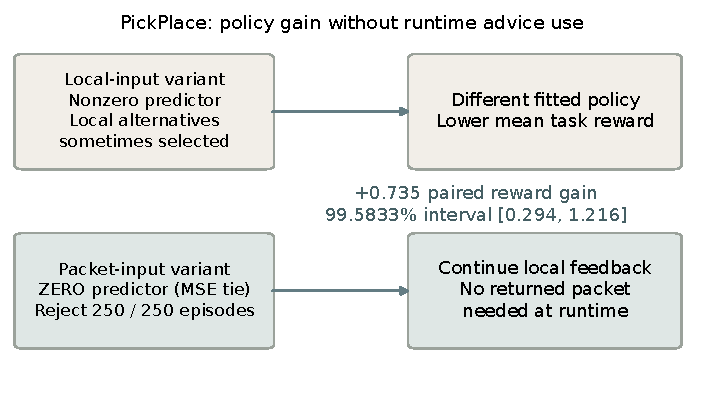
\includegraphics[width=\textwidth]{figures/null_counterexample.pdf}
\caption{PickPlace's positive input-labelled contrast compiles to continued local feedback. The zero predictor wins a validation tie and never accepts an intervention. The performance gap is real for these separately fitted pipelines, but does not establish runtime message value.}\label{fig:visual}
\end{figure}

The original full-policy losses were mostly assigned to selected local alternatives: on Push, 149 local selections contributed $-0.364$, 17 source selections about $-0.001$, and 84 rejects zero to the overall difference. PickPlace's 170 local and 80 source selections contributed $-0.652$ and $+0.016$. This descriptive accounting does not identify effects within selected strata or validate deleting local options after testing. An elapsed-aligned source suffix had positive descriptive differences against reject on both tasks; learned-router loss is not failure of every source action.

\subsection{Direct visual and state message-channel outcomes}\label{sec:channelresults}
The visual bridge completes 60 fresh nonzero-delay PickPlace environments with the original frozen actors and receivers. The nonzero $P,F$ gate changes option after refresh in 10/60 cases; complete action sequences change in 28/60. Its refresh-minus-stale reward difference is $-0.1428$ with approximate 98.3333\% interval $[-0.4932,0.2285]$, leaving a positive refresh benefit unresolved. Stale-minus-absence is $-0.5180$ $[-1.1557,0.0521]$; fresh-minus-absence is $-0.6608$ $[-1.2486,-0.0836]$. Thus the fresh implementation performs below the specified reject fallback in this cohort, while the fresh/stale comparison does not establish benefit or equivalence.

The original null $P,C$ receiver continues to reject under all three channels, with identical trajectories. By contrast, the local-input/full-action receiver changes no option but changes actions in 19/60 cases. This directly demonstrates gate versus actuation dependence in the original visual setting. The $P,C$ counterexample and $P,F$ channel estimate remain different frozen receivers within one actor system, not interchangeable estimands.

The full packet receiver's any-success is 83.3\% stale, 80.0\% fresh and 88.3\% absent; terminal-success is 60.0\%, 61.7\% and 58.3\%. These descriptive endpoints need not rank channels identically. All 177 distinct main-cohort plans retain full trajectories; six separate zero-delay identities and two engineering cases are excluded. Independent replay regenerates request/arrival source packets and features, and every reject tail is checked. The result concerns one task and one trained visual system with its unchanged delay-indexed decoder.

The state study separately executed all 180 fresh environments. For its full packet policy, refreshing changed mean reward by $+0.037667$ on Drawer and $+0.038542$ on Door; both primary intervals include zero (Table~\ref{tab:channel}). This leaves a positive refresh benefit unresolved. It does not prove advice inefficacy or equivalence. Button is different: its selected zero policies structurally reject under all channels. Under the declared absence-to-reject wrapper, stale delivery reduces reward on Drawer and Door. That availability contrast includes the specific fallback and does not establish that expert information is generally harmful.
\begin{table}[tb]\centering\small
\caption{Fixed full packet receiver: primary native reward channel effects. PickPlace uses one frozen visual system and 60 nonzero-delay environments (98.3333\% intervals, family of three). State rows use 60 environments/task including zero delay and five frozen critics (99.5833\%, original family of 12). $S/F/E$ denote stale/fresh/absent; absence invokes the fixed reject wrapper. These distinct regimes are not pooled. Button zeros are structural.}\label{tab:channel}
\setlength{\tabcolsep}{4pt}\begin{tabular}{llrr}\toprule Task / observation & Contrast & Mean & Interval\\\midrule
PickPlace / RGB & $F-S$ & -0.1428 & [-0.4932, +0.2285]\\
PickPlace / RGB & $S-E$ & -0.5180 & [-1.1557, +0.0521]\\
PickPlace / RGB & $F-E$ & -0.6608 & [-1.2486, -0.0836]\\
Drawer / state & $F-S$ & +0.0377 & [-0.0232, +0.2076]\\
Drawer / state & $S-E$ & -0.0756 & [-0.2513, -0.0117]\\
Drawer / state & $F-E$ & -0.0380 & [-0.0728, -0.0127]\\
Door / state & $F-S$ & +0.0385 & [-0.1016, +0.2079]\\
Door / state & $S-E$ & -0.1026 & [-0.2906, -0.0004]\\
Door / state & $F-E$ & -0.0640 & [-0.2148, +0.0003]\\
Button / state & $F-S$ & +0.0000 & [+0.0000, +0.0000]\\
Button / state & $S-E$ & +0.0000 & [+0.0000, +0.0000]\\
Button / state & $F-E$ & +0.0000 & [+0.0000, +0.0000]\\
\bottomrule\end{tabular}\end{table}


Choice and command dependence differ. Among the 300 state environment/critic records per task, $P,F$ changes option under refresh in 62 Drawer and 57 Door records, but complete actions change in 142 and 159. The local-input/full-action selector changes \emph{no} option while actions change in 115 and 114 records: a fixed named source option executes different message values. A gate-only audit misses this path. Door's $P,C$ changes choices and actions in 90/300 records. These are sampled-input diagnostics, not global certificates.

State any-success is identical across channels: 100\% Drawer/Button and 95\% Door. Door terminal-success is 0\%. Only about 30 of 500 steps satisfy its native coordinate-band criterion. Figure~\ref{fig:door-time} shows this transient success alongside sustained shaped reward; flag loss alone does not identify door reclosure. Full duration data and post-hoc nonzero-delay uncertainty are in Online Resource 1. These endpoints answer different questions; reward is not a universally superior objective.


\begin{figure}[tb]\centering
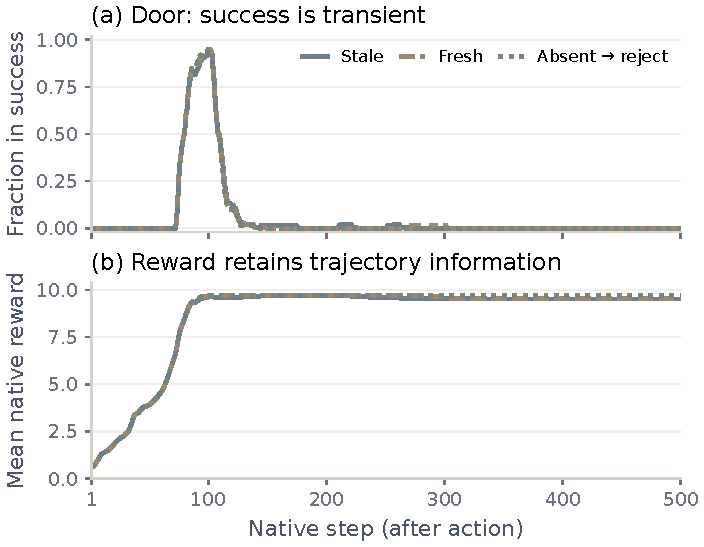
\includegraphics[width=\textwidth]{figures/door_temporal.pdf}
\caption{Door success and native reward under stale, fresh and absent-message channels. Means retain all 60 environments and five frozen $P,F$ critics with environment-equal weighting. Brief success-band occupancy explains the 95\% ever-success/0\% terminal-success discrepancy, while shaped reward remains high. No trajectory selection or timewise inference is used. Full descriptive data are in Online Resource 1.}\label{fig:door-time}
\end{figure}

\subsection{Headroom separates opportunity from harmful selection}\label{sec:headroomresults}
Finite-pool diagnosis reveals two regimes (Table~\ref{tab:headroom}). The visual all-option subset has substantial headroom: 1.285 Push and 1.630 PickPlace, with selector regret 0.978 and 2.396. Some source option exceeds reject by 0.25 in 43.3\% and 36.7\% of the 30 system--environment records/task. Lack of useful candidate actions alone cannot explain these visual failures. However, source-exclusive headroom above the best local option averages only 0.0203 and 0.0913: most available improvement is shared with local alternatives.
\begin{table}[tb]\centering\small
\caption{Distinct finite-pool regimes under stale messages. $H$: full headroom; $H_E$: positive best-source gain; $X$: source-exclusive headroom over the best local option; $G$: full packet selector regret. Visual rows use ten shared initial environments/task across three systems; state rows use 60 environments/task and five critics. No rows are pooled, and no oracle is deployable.}\label{tab:headroom}\label{tab:visualoracle}
\begin{tabular}{llrrrr}\toprule Task & Observation & $H$ & $H_E$ & $X$ & $G$\\\midrule
Push & RGB+robot & 1.2850 & 0.3733 & 0.0203 & 0.9775\\
PickPlace & RGB+robot & 1.6298 & 0.8230 & 0.0913 & 2.3963\\
Drawer & State & 0.00657 & 0.00404 & 0.00150 & 0.08222\\
Door & State & 0.00073 & 0.00048 & 0.00042 & 0.10331\\
Button & State & 0.00026 & 0.00025 & 0.00025 & 0.00026\\\bottomrule
\end{tabular}
\end{table}


The state pool instead offers little average improvement: full-pool headroom is below 0.008 even with refresh, and no stale source option improves by more than 0.25 in any environment. Stale-channel regret on Drawer/Door is much larger than available headroom. Only 24.1\%/2.5\% of selected source actions improve on reject. Drawer source selections contribute $-0.076528$ to the overall $-0.075647$ difference, unlike the local-alternative losses in the original visual cohort. Candidate opportunity and failure mechanism therefore differ by regime; neither diagnosis transfers automatically between them.

The identity $U_\pi-U_R=H-G$ explains how limited opportunity and selection loss coexist. Headroom uses future outcomes and is not deployable performance, nor an information-value upper bound: messages could help select local options. Lowering the state acceptance threshold from $10^{-8}$ to zero changes no recorded choice, so that small threshold does not explain these decisions. State/time strata are descriptive and mix remaining horizon, task state and request time; they do not uniquely identify prediction error or validate a new selector. Full diagnostics remain in Online Resource 1.

\subsection{Complete visual training variation leaves benefit unresolved}\label{sec:fullseedresults}
Three complete systems were evaluated on 100 shared independent initial environments, yielding 300 logical arrival cases plus separate reset-source trajectories. All 1,200 fitted-cell decisions and saved reward means were reproduced, with unchanged model hashes. The full packet policy's difference from reject is $+0.068$ on Push and $-0.382$ on PickPlace; their approximate 99.1667\% intervals cross zero (Table~\ref{tab:fullseeds}). None of the six primary contrasts has a positive lower bound.
\begin{table}[tb]\centering\small
\caption{Complete visual training replication: three independently trained systems, each with a 15,000-update ACT budget, all four local heads and separately fitted arrival critics. Fifty initial environments/task are shared across seeds. These are pipeline contrasts with approximate 99.1667\% crossed-bootstrap intervals (six-contrast family), conditional on the common demonstration corpus and development schedule.}\label{tab:fullseeds}
\begin{tabular}{llrr}\toprule Task & Contrast & Mean & Interval\\\midrule
Push & $P,C-L,C$ & -0.009 & [-0.427, +0.260]\\
Push & $P,F-P,C$ & +0.206 & [-0.066, +0.861]\\
Push & $P,F-R$ & +0.068 & [-0.593, +0.722]\\
PickPlace & $P,C-L,C$ & +0.426 & [-0.367, +1.600]\\
PickPlace & $P,F-P,C$ & -0.361 & [-1.526, +0.000]\\
PickPlace & $P,F-R$ & -0.382 & [-1.500, +0.319]\\
\bottomrule\end{tabular}\end{table}


The PickPlace input contrast is $+0.426$ $[-0.367,1.600]$, qualifying transfer of the original positive pipeline result across training randomness. Seed 0's exact null $P,C$ again rejects all 50 new cases; the other 23 input/action/task/seed cells are nonzero. These correlated cells do not estimate a population null-selection frequency. Push seed 1 has a $+0.379$ full-policy point difference with all 50 interventions assigned to local alternatives; its nonzero packet gate could still use messages to route among them. Absence of source actuation is not independence. Per-seed contrasts and complete-source competence, including all weak outcomes, are retained only in Online Resource 1, Tables S8--S9. The systems share data, pretraining and development arrangements, so this is conditional training variation, not cross-dataset generalization.

\subsection{Generation-time decoding and the frozen selector differ}\label{sec:decoderresults}
Matching generation time improves the predefined fresh 48-step chunk relative to applying its old delay offset: the paired mean gain is 0.579 (Table~\ref{tab:decoder}). This establishes an execution-index effect for that fixed option in the new cohort. Its time-matched fresh versus stale difference remains unresolved, as does its descriptive advantage over continued local control ($+0.120$, 95\% interval $[-0.187,0.433]$). Improvement in this decoder comparison does not by itself establish a useful refresh channel or an overall advice advantage.
\begin{table}[tb]\centering\small
\caption{Independent generation-time decoding control: four primary reward contrasts on 60 new environments. Time uses generation age; legacy uses request delay. Stale decoding is identical for both. Approximate 98.75\% stratified paired-bootstrap intervals retain the four-contrast family. Fixed48 applies the predefined source suffix on every environment; the frozen gate uses unchanged choices across fresh decoders. This study does not alter the original channel estimates.}\label{tab:decoder}
\setlength{\tabcolsep}{3pt}\begin{tabular}{llrr}\toprule Receiver & Contrast & Mean & Interval\\\midrule
Fixed48 & Fresh: time $-$ legacy & +0.579 & [+0.173, +0.997]\\
Fixed48 & Time-fresh $-$ stale & +0.149 & [-0.204, +0.516]\\
Frozen $P,F$ & Fresh: time $-$ legacy & -0.030 & [-0.298, +0.192]\\
Frozen $P,F$ & Time-fresh $-$ stale & -0.188 & [-0.541, +0.116]\\
\bottomrule\end{tabular}\end{table}


The frozen $P,F$ gate responds differently. It chooses a suffix in 24/60 environments (21 for 48 steps and three for 16), so time matching changes 24 action sequences while changing no fresh-channel choice. Its mean decoder effect is $-0.030$, with a primary interval crossing zero. Local-option selections are unaffected. The fixed option's overall gain therefore does not transfer automatically to the gate's selected states and intervention lengths. The gate still predicts legacy-execution gains; this study does not test learning or recalibrating it for the new rule. Complete channel/decoder outcomes, success endpoints and index checks are in Online Resource 1.

These new results qualify a practical reading of the earlier channel test: literal replacement in the legacy receiver and generation-matched execution answer different questions. We retain both, with separate environments, receivers and inference families. The positive fixed-chunk decoder result is not used to relabel the original refresh effect or the packet-independent $+0.735$ counterexample.

\subsection{Supporting analyses bound rather than erase the counterexample}\label{sec:toleranceresults}
The independent critic-data curve uses 7/14/28 nested training episodes with fixed validation. All 24 selected models are nonzero. At 28 episodes, $P,F-R$ is $+0.013$ on Push and $-0.087$ on PickPlace; neither interval establishes benefit. The single nested draw does not prove that more data or a different selector cannot help.

Selection tolerance and deployment threshold have different roles. Across the same 100 development resplits, PickPlace $P,C$ selects zero in 13/14/17/19/19 cases at tie tolerances $0/10^{-14}/10^{-12}/10^{-10}/10^{-8}$. Null prevalence depends on the selection rule and split. The original $+0.735$ estimate is conditional on that rule; the strict-MSE alternative is a different policy whose test effect was not measured. The frozen zero policy's exact independence, and the logical failure of pipeline gain to establish channel value, do not require zero to be commonly selected.

The 360-environment state stress suite varies delay, frequency and noise. It establishes no positive packet/local-input advantage; full policies lose reward on Drawer/Door while Button structurally rejects. Door's zero-packet probe changes 70.9\% of $P,C$ choices, but lacks rerolled outcomes and may be outside training support. It is sensitivity evidence only. All primary contrasts, condition tables, curves, tolerance grids and historical source-budget results remain in Online Resource 1. None is used for test-driven retuning.

\section{Discussion}\label{sec:discussion}
The strongest finding is an attribution failure that survives accurate reward measurement: a positive packet-input-labelled pipeline contrast was implemented by a policy that did not need the runtime packet. The visual and state fixed-policy channel experiments complete a different part of the evidence chain. They execute defined message interventions and measure their outcomes, rather than inferring value from input sensitivity. Refreshing changes some choices and many action sequences, but does not establish positive mean reward value for these policies. These are distinct results, not successive estimates of one interchangeable quantity.

Retained expertise remains compatible with the null certificate. Students can embody teacher knowledge through demonstrations, memory and learned representations~\cite{zhu,ilhan,silva}. Our visual policies share a pretrained encoder, and the state source's inputs are also public to the local agent. A deterministic transformation may still save computation or help a restricted model even without private Shannon information. Conversely, including that transformation in a fitted feature vector does not show that the selected deployed policy consumes it. An exact null certificate resolves the latter dependency question; it does not measure a complete system's historical dependence on expertise.

The headroom analysis refines the explanation of intervention failure. The visual subset offers substantial finite-pool improvement, so strong baseline competence is not a sufficient explanation there. Much of that opportunity is shared by local alternatives, and the selector leaves it unrealized. In the new state cohort, local behavior meeting the declared ever-success criterion leaves small reward improvements within the declared source family, while the selector can still incur appreciable downside. In the original visual cohort, selected local alternatives account for most loss. Neither the existence of a tiny positive source gain nor a capable complete-episode expert guarantees a useful occasional repair. The exact finite-pool decomposition separates available opportunity from selection regret, but does not uniquely attribute failure to representation, prediction error or action-family design. A wider action family might increase both opportunity and selection risk. Testing such a remedy requires new development data and held-out evaluation, not deletion of harmful options after seeing test outcomes.

The independent decoder control shows why freezing weights alone does not define a fixed executable policy. A generation-matched index improves the predefined fresh chunk relative to retaining its stale offset, while the same change does not establish a benefit for the frozen selector. The gate uses a different state/option distribution and still predicts legacy outcomes. Thus a decoder correction can remove one execution mismatch without validating a learned acceptance mechanism. A further acceptance-policy study would require new development labels under the corrected semantics and fresh held-out evaluation; the present test supplies neither retraining nor an optimized controller.

\subsection{Implications for the evaluation of autonomous agents}\label{sec:implications}
The framework can guide evaluation in several potential applications. For a robot consulting a remote expert, define the observation timestamp used to generate the reply, what the robot does while waiting, and whether a refreshed reply incurs additional latency. Record message-generation time separately from elapsed request delay and specify how the executor converts it to an action-chunk index. Keep the deployed receiver fixed when comparing delivery mechanisms. Report both the gate's decision and the actuator commands, because unchanged option labels can conceal message-driven execution. A simulator with verified restoration can supply paired outcomes; the present experiments validate this route only in the specified simulation setup.

For human corrections, the message mechanism must additionally specify teacher access, semantics and the absence rule. A random numerical packet is not necessarily a plausible human alternative. Human attention, learning and adaptation may change across conditions, making a fixed teacher or fixed receiver assumption inappropriate. The framework's three questions remain useful for designing such a study, but our scripted source does not validate human-advice effectiveness or the required behavioral assumptions.

For a cloud policy advising an edge controller, distinguish newly delivered content from expertise already distilled into the edge model. A null runtime receiver may still depend on cloud-generated training data. Comparing large/small or high/low-compute agents also requires accounting for invocation frequency, communication and fallback cost. A deployment study should estimate its own complete cost-aware channel contrast.

A transferable minimum report therefore identifies the fixed receiver or update algorithm, message provider and conditioning, candidate rules, fallback, clock and cost model, dependence paths, and outcome estimator. Without rollback, randomized live comparisons or justified logged-data evaluation are needed~\cite{dudik,jiang,thomas}; decision substitution alone supplies no missing trajectory outcomes. For a continually learning receiver, the frozen object would have to be the complete update procedure and its initialization, not a single checkpoint. Those settings are potential extensions, not validated applications of the present code.

\subsection{External validity and unresolved uncertainty}
The distinction between pipeline and channel contrasts is general, while the measurements are local to the tested systems. All five tasks use one simulator family. Push and PickPlace use visual ACT and learned heads; Drawer, Door and Button use state observations, public scripted sources and local behavioral cloning. This broadens contact mechanics without establishing five-task visual-model performance. Native channel value is measured in three state/public-source tasks and one frozen visual PickPlace system. The new visual bridge connects the observation and actor setting of the original counterexample to an actual channel intervention, but the null $P,C$ and nonzero $P,F$ receivers are different policies. It does not identify the original input-labelled gap as message value, nor provide a multi-seed visual-channel replication. Navigation, language advice, private expert observations and strategic multi-agent interaction are untested.

The refreshed channel is generated by a real permitted source computation, but changes its joint relation to critic inputs compared with stale-only training. Its native effect is interpretable as this controlled refresh intervention, not as an unrestricted measure of expert information. The missing-message comparison also includes our predeclared absence-to-reject wrapper; it is not evidence of a learned missing-input capability. The independent decoder study additionally assumes a known, correct generation timestamp and changes the downstream rule while keeping a legacy-trained gate. It bounds an execution mismatch in one visual system, not the best achievable timestamp-aware policy. No additional refresh latency or service cost is charged, so neither study supplies net acquisition value.

Training variation is now tested through three complete visual systems, each with a 15k-update source budget, all four local heads and separately fitted arrival critics. The original 500-environment counterexample remains one accepted system; its null policy also rejected all 50 new PickPlace cases, while the new seed-1/2 models were nonzero. The pooled visual benefit remained unresolved, and only one of the three Push full-policy point differences was positive. These systems share a demonstration corpus, pretrained initialization, capacities and development schedule, so they assess conditional training randomness, not new datasets or pretraining distributions. Three actor seeds and five state critic seeds still give limited training-population coverage. Development resplits likewise reuse episodes and are not independent performance tests. An exact certificate for a frozen null policy and the prevalence of such policies remain separate questions.

The attribution distinction is not unique to latency. Delay adds decisions about message-generation timestamps, arrival state, continuation and request clocks that must be specified before a channel comparison is interpretable. Synthetic native-step delays and Gaussian coordinate noise do not reproduce a live asynchronous service, human misunderstanding or real network contention. Fixed requests do not evaluate a learned acquisition policy. No physical robot is used. Consequently, the experiments establish no hardware safety guarantee. Shared random streams and bitwise restoration are verified on this machine under recorded versions and renderer settings; clean-machine and independent external reproduction remain separate checks. Local weights, data and traces must be included in a verified archival release before public availability can be claimed. Human authors must verify interpretation, release permissions and submission declarations.

\section{Conclusion}
The framework makes three advice-evaluation questions independently executable: how fitted pipelines perform, whether frozen behavior depends on the returned message, and what outcomes change under a specified message channel. The positive visual pipeline counterexample required no runtime packet. Native channel interventions then showed that message-sensitive decisions and actions did not establish positive refresh value, while finite-pool diagnostics separated limited opportunity from harmful selection. The practical contribution is a reproducible route from a performance claim to a bounded attribution conclusion, not a universally superior acceptance controller or a general claim that expert advice is ineffective.

\section*{Statements and Declarations}
\paragraph{Author approval and responsibility.}
Junxiang Wang and Jiaoyang Su have reviewed and approved the manuscript and its submission. Both authors take responsibility for the work.
\paragraph{Funding.}
No funding was received for this research.
\paragraph{Competing interests.}
The authors declare no competing interests.
\paragraph{Data and code availability.}
The source code and analyzed data supporting this study are maintained in the project's GitHub repository. The analyzed source data also accompany this submission.
\paragraph{Ethics and consent.}
This study uses simulated robotic tasks and computational advisors; it involves no human participants, animals or physical robot experiments.
\paragraph{Prior publication.}
This manuscript has not been published previously and is not under consideration elsewhere. There are no related prior publications or preprints.
\paragraph{Use of AI tools.}
OpenAI Codex assisted code development, experiment execution, analysis and manuscript drafting. Both authors reviewed and approved the manuscript and take responsibility for its content.

\begin{thebibliography}{99}
\bibitem{fachantidis} Fachantidis, A., Taylor, M. E., \& Vlahavas, I. (2019). Learning to teach reinforcement learning agents. \emph{Machine Learning and Knowledge Extraction}, 1(1), 21--42. \url{https://doi.org/10.3390/make1010002}
\bibitem{najar} Najar, A., \& Chetouani, M. (2021). Reinforcement learning with human advice: A survey. \emph{Frontiers in Robotics and AI}, 8, 584075. \url{https://doi.org/10.3389/frobt.2021.584075}
\bibitem{chernova} Chernova, S., \& Veloso, M. (2009). Interactive policy learning through confidence-based autonomy. \emph{Journal of Artificial Intelligence Research}, 34, 1--25. \url{https://doi.org/10.1613/jair.2584}
\bibitem{zhu} Zhu, C., Cai, Y., Hu, S., Leung, H.-f., \& Chiu, D. K. W. (2023). Learning by reusing previous advice: A memory-based teacher--student framework. \emph{Autonomous Agents and Multi-Agent Systems}, 37, Article 14. \url{https://doi.org/10.1007/s10458-022-09595-1}
\bibitem{ilhan} \.{I}lhan, E., Gow, J., \& Perez-Liebana, D. (2021). Action advising with advice imitation in deep reinforcement learning. In \emph{Proceedings of the 20th International Conference on Autonomous Agents and Multiagent Systems} (pp. 629--637). \url{https://www.ifaamas.org/Proceedings/aamas2021/pdfs/p629.pdf}
\bibitem{act} Zhao, T. Z., Kumar, V., Levine, S., \& Finn, C. (2023). Learning fine-grained bimanual manipulation with low-cost hardware. In \emph{Proceedings of Robotics: Science and Systems XIX}. \url{https://doi.org/10.15607/RSS.2023.XIX.016}
\bibitem{rtc} Black, K., Galliker, M. Y., \& Levine, S. (2025). Real-time execution of action chunking flow policies. \emph{Advances in Neural Information Processing Systems}, 38. \url{https://doi.org/10.52202/085713-1122}
\bibitem{silva} da Silva, F. L., \& Costa, A. H. R. (2019). A survey on transfer learning for multiagent reinforcement learning systems. \emph{Journal of Artificial Intelligence Research}, 64, 645--703. \url{https://doi.org/10.1613/jair.1.11396}
\bibitem{agarwal} Agarwal, R., Schwarzer, M., Castro, P. S., Courville, A. C., \& Bellemare, M. G. (2021). Deep reinforcement learning at the edge of the statistical precipice. \emph{Advances in Neural Information Processing Systems}, 34, 29304--29320. 
\bibitem{pineau} Pineau, J., Vincent-Lamarre, P., Sinha, K., Larivi\`ere, V., Beygelzimer, A., d'Alch\'e-Buc, F., Fox, E., \& Larochelle, H. (2021). Improving reproducibility in machine learning research (a report from the NeurIPS 2019 reproducibility program). \emph{Journal of Machine Learning Research}, 22(164), 1--20. \url{https://jmlr.org/papers/v22/20-303.html}
\bibitem{metaworld} Yu, T., Quillen, D., He, Z., Julian, R., Hausman, K., Finn, C., \& Levine, S. (2020). Meta-World: A benchmark and evaluation for multi-task and meta reinforcement learning. \emph{Proceedings of Machine Learning Research}, 100, 1094--1100. \url{https://proceedings.mlr.press/v100/yu20a.html}

\bibitem{torrey} Torrey, L., \& Taylor, M. E. (2013). Teaching on a budget: Agents advising agents in reinforcement learning. In \emph{Proceedings of AAMAS} (pp. 1053--1060). \url{https://www.ifaamas.org/Proceedings/aamas2013/docs/p1053.pdf}
\bibitem{taylor} Taylor, M. E., \& Stone, P. (2009). Transfer learning for reinforcement learning domains: A survey. \emph{Journal of Machine Learning Research}, 10(56), 1633--1685. \url{https://jmlr.org/papers/v10/taylor09a.html}
\bibitem{griffith} Griffith, S., Subramanian, K., Scholz, J., Isbell, C. L., \& Thomaz, A. L. (2013). Policy shaping: Integrating human feedback with reinforcement learning. \emph{Advances in Neural Information Processing Systems}, 26. 
\bibitem{macglashan} MacGlashan, J., Ho, M. K., Loftin, R., Peng, B., Wang, G., Roberts, D. L., Taylor, M. E., \& Littman, M. L. (2017). Interactive learning from policy-dependent human feedback. \emph{Proceedings of Machine Learning Research}, 70, 2285--2294. \url{https://proceedings.mlr.press/v70/macglashan17a.html}
\bibitem{celemin} Celemin, C., \& Ruiz-del-Solar, J. (2019). An interactive framework for learning continuous actions policies based on corrective feedback. \emph{Journal of Intelligent \& Robotic Systems}, 95(1), 77--97. \url{https://doi.org/10.1007/s10846-018-0839-z}
\bibitem{dulac} Dulac-Arnold, G., Levine, N., Mankowitz, D. J., Li, J., Paduraru, C., Gowal, S., \& Hester, T. (2021). Challenges of real-world reinforcement learning: Definitions, benchmarks and analysis. \emph{Machine Learning}, 110(9), 2419--2468. \url{https://doi.org/10.1007/s10994-021-05961-4}
\bibitem{ramstedt} Ramstedt, S., \& Pal, C. (2019). Real-time reinforcement learning. \emph{Advances in Neural Information Processing Systems}, 32. 
\bibitem{randomdelay} Bouteiller, Y., Ramstedt, S., Beltrame, G., Pal, C., \& Binas, J. (2021). Reinforcement learning with random delays. In \emph{International Conference on Learning Representations}. \url{https://openreview.net/forum?id=QFYnKlBJYR}
\bibitem{diffusion} Chi, C., Feng, S., Du, Y., Xu, Z., Cousineau, E., Burchfiel, B. C., \& Song, S. (2023). Diffusion policy: Visuomotor policy learning via action diffusion. In \emph{Robotics: Science and Systems XIX}. \url{https://doi.org/10.15607/RSS.2023.XIX.026}
\bibitem{ross} Ross, S., Gordon, G., \& Bagnell, D. (2011). A reduction of imitation learning and structured prediction to no-regret online learning. \emph{Proceedings of Machine Learning Research}, 15, 627--635. \url{https://proceedings.mlr.press/v15/ross11a.html}
\bibitem{jiang} Jiang, N., \& Li, L. (2016). Doubly robust off-policy value evaluation for reinforcement learning. \emph{Proceedings of Machine Learning Research}, 48, 652--661. \url{https://proceedings.mlr.press/v48/jiang16.html}
\bibitem{thomas} Thomas, P., \& Brunskill, E. (2016). Data-efficient off-policy policy evaluation for reinforcement learning. \emph{Proceedings of Machine Learning Research}, 48, 2139--2148. \url{https://proceedings.mlr.press/v48/thomasa16.html}
\bibitem{swaminathan} Swaminathan, A., \& Joachims, T. (2015). Counterfactual risk minimization: Learning from logged bandit feedback. \emph{Proceedings of Machine Learning Research}, 37, 814--823. \url{https://proceedings.mlr.press/v37/swaminathan15.html}
\bibitem{dudik} Dud\'ik, M., Erhan, D., Langford, J., \& Li, L. (2014). Doubly robust policy evaluation and optimization. \emph{Statistical Science}, 29(4), 485--511. \url{https://doi.org/10.1214/14-STS500}
\bibitem{cawley} Cawley, G. C., \& Talbot, N. L. C. (2010). On over-fitting in model selection and subsequent selection bias in performance evaluation. \emph{Journal of Machine Learning Research}, 11(70), 2079--2107. \url{https://jmlr.org/papers/v11/cawley10a.html}
\bibitem{varma} Varma, S., \& Simon, R. (2006). Bias in error estimation when using cross-validation for model selection. \emph{BMC Bioinformatics}, 7, 91. \url{https://doi.org/10.1186/1471-2105-7-91}
\bibitem{henderson} Henderson, P., Islam, R., Bachman, P., Pineau, J., Precup, D., \& Meger, D. (2018). Deep reinforcement learning that matters. \emph{Proceedings of the AAAI Conference on Artificial Intelligence}, 32(1). \url{https://doi.org/10.1609/aaai.v32i1.11694}
\bibitem{fisher} Fisher, A., Rudin, C., \& Dominici, F. (2019). All models are wrong, but many are useful: Learning a variable's importance by studying an entire class of prediction models simultaneously. \emph{Journal of Machine Learning Research}, 20(177), 1--81. \url{https://jmlr.org/papers/v20/18-760.html}
\bibitem{hooker} Hooker, G., Mentch, L., \& Zhou, S. (2021). Unrestricted permutation forces extrapolation: Variable importance requires at least one more model, or there is no free variable importance. \emph{Statistics and Computing}, 31(6), 82. \url{https://doi.org/10.1007/s11222-021-10057-z}
\bibitem{strobl} Strobl, C., Boulesteix, A.-L., Kneib, T., Augustin, T., \& Zeileis, A. (2008). Conditional variable importance for random forests. \emph{BMC Bioinformatics}, 9, 307. \url{https://doi.org/10.1186/1471-2105-9-307}
\end{thebibliography}

\end{document}
